%-------------------------------
%	PACKAGES AND OTHER DOCUMENT CONFIGURATIONS
%-------------------------------

% The \vref command specifies the location of the reference

%\documentclass[
%10pt, % Main document font size
%a4paper, % Paper type, use 'letterpaper' for US Letter paper
%oneside, % One page layout (no page indentation)
%twoside, % Two page layout (page indentation for binding and different headers)
%headinclude,footinclude, % Extra spacing for the header and footer
%BCOR5mm, % Binding correction
%]{scrartcl}


\documentclass{article}


%--------------------------------------------------------------
%	REQUIRED PACKAGES
%--------------------------------------------------------------

\usepackage[
nochapters, % Turn off chapters since this is an article        
beramono, % Use the Bera Mono font for monospaced text (\texttt)
%eulermath,% Use the Euler font for mathematics
pdfspacing, % Makes use of pdftex’ letter spacing capabilities via the microtype package
dottedtoc % Dotted lines leading to the page numbers in the table of contents
]{classicthesis} % The layout is based on the Classic Thesis style



\usepackage{arsclassica} % Modifies the Classic Thesis package

\usepackage[T1]{fontenc} % Use 8-bit encoding that has 256 glyphs

\usepackage[utf8]{inputenc} % Required for including letters with accents
%--------------------------------------------------------------
% Fonts and languages
\usepackage{libertinus} % The Libertinus font
%\usepackage[adobe-utopia]{mathdesign} % The Utopia font
%\usepackage[p,osf]{scholax}
% T1 and textcomp are loaded by package. Change that here, if you want
% load sans and typewriter packages here, if needed
%\usepackage{amsmath,amsthm}% must be loaded before newtxmath
% amssymb should not be loaded
%\usepackage[scaled=1.075,ncf,vvarbb]{newtxmath}% need to scale up math package
% vvarbb selects the STIX version of blackboard bold.


\usepackage[czech]{babel} % Český jazyk
%--------------------------------------------------------------
\usepackage{graphicx} % Required for including images
\graphicspath{{Figures/}} % Set the default folder for images

\usepackage{enumitem} % Required for manipulating the whitespace between and within lists

\usepackage{lipsum} % Used for inserting dummy 'Lorem ipsum' text into the template

\usepackage{subfig} % Required for creating figures with multiple parts (subfigures)

\usepackage{amsmath,amssymb,amsthm,amsfonts} % For including math equations, theorems, symbols, etc

\usepackage{varioref} % More descriptive referencing

\usepackage[top =3 cm, bottom = 3.5 cm, left = 1.5 cm, right = 1.5 cm]{geometry}

\usepackage{mathtools}

\usepackage{float}

\usepackage{caption}

%------------------------------------------------------------
%	DIAGRAMS AND TIKZ
\usepackage{smartdiagram}
\usepackage{metalogo}
\usepackage{tikz}
\usetikzlibrary{matrix,calc}

\usepackage{hhline} % kvůli double line v tabulkách
%------------------------------------------------------------
%	THEOREM STYLES
%------------------------------------------------------------

\theoremstyle{definition} % Define theorem styles here based on the definition style (used for definitions and examples)
\newtheorem{definition}{Definice}
\newtheorem{example}{Příklad}
\newtheorem{exercise}{Cvičení}

\theoremstyle{plain} % Define theorem styles here based on the plain style (used for theorems, lemmas, propositions)
\newtheorem{theorem}{Věta}

\theoremstyle{remark} % Define theorem styles here based on the remark style (used for remarks and notes)
\newtheorem{remark}{Poznámka}



%-------------------------------------------------------------
%	HYPERLINKS
%-------------------------------------------------------------

\hypersetup{
%draft, % Uncomment to remove all links (useful for printing in black and white)
colorlinks=true, breaklinks=true, bookmarks=true,bookmarksnumbered,
urlcolor=webbrown, linkcolor=RoyalBlue, citecolor=webgreen, % Link colors
pdftitle={}, % PDF title
pdfauthor={\textcopyright}, % PDF Author
pdfsubject={}, % PDF Subject
pdfkeywords={}, % PDF Keywords
pdfcreator={pdfLaTeX}, % PDF Creator
pdfproducer={LaTeX with hyperref and ClassicThesis} % PDF producer
}

 % Include the structure.tex file which specified the document structure and layout

%----------------------------------------------------
%	MATHEMATICS
%----------------------------------------------------

% Tělesa, obory íntegrity a metrické prostory
\newcommand{\C}{\mathbb{C}}
\newcommand{\R}{\mathbb{R}}
\newcommand{\N}{\mathbb{N}}
\newcommand{\Q}{\mathbb{Q}}
\newcommand{\Z}{\mathbb{Z}}
\renewcommand{\L}[2]{L^{#1} \left( #2 \right)} % Lebesgueovy prostory

\newcommand{\vc}[1]{\boldsymbol{#1}} % vektor
\newcommand{\mat}[1]{\mathbf{#1}} % matice

\newcommand{\norm}[1]{\left \Vert #1 \right \Vert} % norma vektoru
\newcommand{\set}[1]{ \left \lbrace #1 \right \rbrace} % množina
\newcommand{\const}{\mathrm{konst}} % konstanta

\newcommand{\F}{\mathcal{F} } % Fourierova transformace
\newcommand{\La}{\mathcal{L}} % Laplaceova transformace

% Označení funkcí
\newcommand{\Res}[2]{\mathrm{Res}_{#1} \, #2 \,} % residuum
\newcommand{\sgn}{\, \mathrm{sign} \,} % signum
\newcommand{\tg}{\,\mathrm{tg}\,} % možné značení tangens


%Značení derivací a integrálů
\newcommand{\der}[2]{\frac{\mathrm{d}#1}{\mathrm{d}#2}} % obyčejná derivace
\newcommand{\pder}[2]{\frac{\partial #1}{\partial #2}} % parciální derivace
\newcommand{\tder}[3]{\left( \pder{#1}{#2} \right)_{#3 = \const}} % termodynamická derivace
\newcommand{\D}{\mathrm{d} } % integrační znamení
\newcommand{\DD}{\mathrm{D}} % absolutní derivace
\newcommand{\intR}{\int_{-\infty}^{\infty}} % integrál přes reálnou osu



% Značení posloupností, limit a sum
\newcommand{\sequence}[2]{ \left \lbrace #1 \right \rbrace_{#2=1}^\infty} % posloupnost
\newcommand{\sumnorm}[1]{\sum_{#1}^\infty} 
\newcommand{\limplus}[1]{\lim_{#1 \rightarrow + \infty}}
\newcommand{\limminus}[1]{\lim_{#1 \rightarrow - \infty}}


% VŠE záležitosti
\newcommand{\dder}[2]{\frac{\Delta #1}{\Delta #2}}


\newcommand{\arctg}{\mathrm{arctg}\,}
\newcommand{\cotg}{\mathrm{cotg}\,}
\newcommand{\arccotg}{\mathrm{arccotg}\,} % Include the mathematics.tex file which uses some mathematical operators

\hyphenation{Fortran hy-phen-ation} % Specify custom hyphenation points in words with dashes where you would like hyphenation to occur, or alternatively, don't put any dashes in a word to stop hyphenation altogether

%-------------------------------
%	TITLE AND AUTHOR(S)
%-------------------------------

%\title{\normalfont\spacedallcaps{Article Title}} % The article title

%\subtitle{Subtitle} % Uncomment to display a subtitle

\author{\spacedlowsmallcaps{Miroslav Burýšek*}} % The article author(s) - author affiliations need to be specified in the AUTHOR AFFILIATIONS block

\date{\today} % An optional date to appear under the author(s)




%-------------------------------------
%	TESTING
%-------------------------------------
% Load packages for testing
\usepackage{blindtext}
%\usepackage{showframe} % Uncomment to show boxes around the text area, margin, header and footer
%\usepackage[inline]{showlabels}  \showlabels[\small\color{JungleGreen}]{}  % Uncomment to output the content of \label commands to the document where they are used


\begin{document}

%-------------------------------------------
%	HEADERS
%-------------------------------------------

\renewcommand{\sectionmark}[1]{\markright{\spacedlowsmallcaps{#1}}} % The header for all pages (oneside) or for even pages (twoside)
%\renewcommand{\subsectionmark}[1]{\markright{\thesubsection~#1}} % Uncomment when using the twoside option - this modifies the header on odd pages
\lehead{\mbox{\llap{\small\thepage\kern1em\color{halfgray} \vline}\color{halfgray}\hspace{0.5em}\rightmark\hfil}} % The header style

\pagestyle{scrheadings} % Enable the headers specified in this block





%-----------------------------------------
%	TABLE OF CONTENTS & LISTS OF FIGURES AND TABLES
%-----------------------------------------

%\maketitle % Print the title/author/date block

\setcounter{tocdepth}{2} % Set the depth of the table of contents to show sections and subsections only

%\tableofcontents % Print the table of contents

%\listoffigures % Print the list of figures

%\listoftables % Print the list of tables






%--------------------------------------
%	ABSTRACT
%--------------------------------------

%\section*{Abstract} % This section will not appear in the table of contents due to the star (\section*)


%---------------------------------------
%	AUTHOR AFFILIATIONS
%---------------------------------------

\let\thefootnote\relax\footnotetext{\textbf{Verze:} \today }

%--------------------------------------

%\newpage % Start the article content on the second page, remove this if you have a longer abstract that goes onto the second page

\section*{Úvod do analýzy funkcí}
\subsection*{Růst a pokles funkce}
O funkci $f$ řekneme, že je \begin{itemize}
    \item \textbf{rostoucí} na intervalu $I$, jestliže pro všechna $x,y \in I$ splňující $x<y$ platí $f(x) < f(y)$,
    \item \textbf{klesající} na intervalu $I$, jestliže pro všechna $x,y \in I$ splňující $x<y$ platí $f(x) < f(y)$,
    \item \textbf{neklesající} na intervalu $I$, jestliže pro všechna $x,y \in I$ splňující $x<y$ platí $f(x) \leq f(y)$,
    \item \textbf{nerostoucí} na intervalu $I$, jestliže pro všechna $x,y \in I$ splňující $x<y$ platí $f(x) \geq f(y)$,
    \item \textbf{monotónní} na intervalu $I$, jestliže je na něm neklesající, anebo nerostoucí,
    \item \textbf{konstantní} na intervalu $I$, jestliže pro všechna $x,y \in I$ splňující $x<y$ platí $f(x) = f(y)$.
\end{itemize}

\begin{figure}[H]
    \centering
    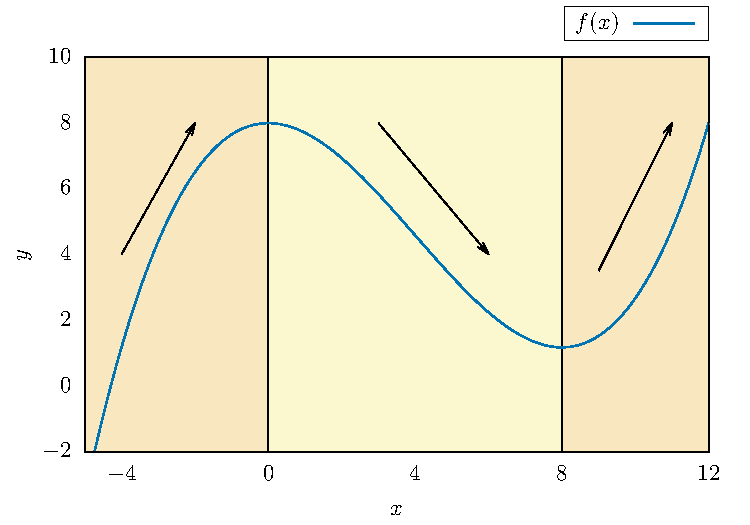
\includegraphics[scale = 0.7]{Gnuplot/Figures/funkce-rostouci-klesajici-obr.pdf}
    \caption{Ilustrace pojmu rostoucí a klesající funkce. Na oranžové oblasti je $f(x)$ rostoucí, na žluté oblasti je $f(x)$ klesající.}
\end{figure}

\begin{remark}
    Pokud mluvíme o růstu nebo poklesu funkce, je vždy nutné uvést, na jakém intervalu se pohybujeme. Důležitost je vidět na následujícím příkladu, viz obrázek \ref{fig:1a-funkce-ne}.

    \begin{figure}[H]
        \centering
        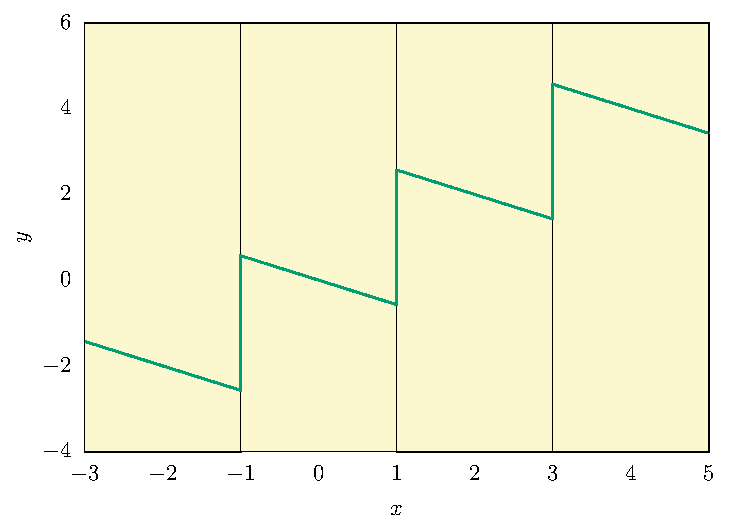
\includegraphics[scale = 0.7]{Gnuplot/Figures/periodicka-klesajici.pdf}
        
        \caption{Příklad funkce, která je klesající na každém intervalu $I_p = (2p-1,2p+1)$, kde $p \in \Z$. Na celém $\R$ ale není ani rostoucí, ani klesající. Porovnáme-li dva body $x_1 < x_2$ v témže intervalu $I_p$, splňují $f(x_1) > f(x_2)$. Porovnáme-li však body v různých intervalech, dostaneme $f(x_1) < f(x_2)$. Není tedy splněna ani jedna z podmínek pro růst nebo pokles na $\R$. Všimněme si, že funkce je v krajních bodech intervalů nespojitá, má v nich skoky.}
        \label{fig:1a-funkce-ne}
    \end{figure}

\end{remark}

\begin{remark}
    V některé literatuře se o různých křivkách mluví jako o \uv{rostoucích zleva doprava} nebo \uv{klesajících zprava doleva} a podobně. Matematická terminologie vždy pracuje s tím, co se děje s hodnotami $f(x)$ \underline{při rostoucích $x$} - tedy vždy \uv{zleva doprava}, chcete-li. Podobně se někdy říká o klesajících funkcích $y(x)$, že \uv{$y$ je nepřímo úměrné $x$}. Ale matematická terminologie říká, že pouze funkce $y(x)=C/x$ je nepřímá úměrnost, žádná jiná funkce toto nesplňuje.

    \begin{figure}[H]
        \centering
        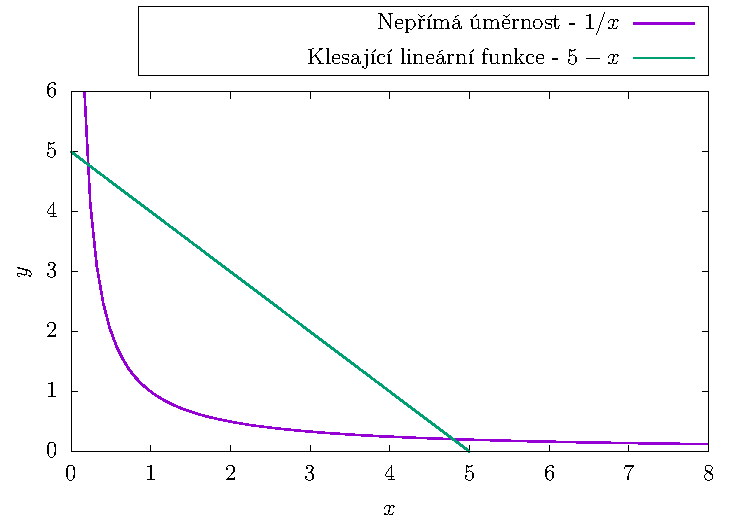
\includegraphics[scale = 0.7]{Gnuplot/Figures/neprima-umernost.pdf}
        \caption{Ilustrace často nesprávně použitého termínu \uv{nepřímá úměrnost}. Pouze funkce typu $C/x$ jsou nepřímé úměrnosti.}
    \end{figure}
\end{remark}

\subsection*{Další charakteristiky funkce}

O funkci $f(x)$ říkáme, že je \begin{itemize}
    \item \textbf{prostá} na intervalu $I$, jestliže pro všechna $x,y \in I$ splňující $x \neq y$ platí $f(x) \neq f(y)$ (\uv{každému $x$ přísluší jiná hodnota $f(x)$}),
    \item \textbf{omezená shora}, jestliže existuje konečné číslo $K$ takové, že pro všechna $x \in D(f)$ platí $f(x) \leq K$,
    \item \textbf{omezená zdola}, jestliže existuje konečné číslo $K$ takové, že pro všechna $x \in D(f)$ platí $f(x) \geq K$,
    \item \textbf{omezená}, jestliže je omezená shora i zdola.
\end{itemize}



\end{document}